% Options for packages loaded elsewhere
\PassOptionsToPackage{unicode}{hyperref}
\PassOptionsToPackage{hyphens}{url}
%
\documentclass[
]{report}
\usepackage{amsmath,amssymb}
\usepackage{lmodern}
\usepackage{iftex}
\ifPDFTeX
  \usepackage[T1]{fontenc}
  \usepackage[utf8]{inputenc}
  \usepackage{textcomp} % provide euro and other symbols
\else % if luatex or xetex
  \usepackage{unicode-math}
  \defaultfontfeatures{Scale=MatchLowercase}
  \defaultfontfeatures[\rmfamily]{Ligatures=TeX,Scale=1}
\fi
% Use upquote if available, for straight quotes in verbatim environments
\IfFileExists{upquote.sty}{\usepackage{upquote}}{}
\IfFileExists{microtype.sty}{% use microtype if available
  \usepackage[]{microtype}
  \UseMicrotypeSet[protrusion]{basicmath} % disable protrusion for tt fonts
}{}
\makeatletter
\@ifundefined{KOMAClassName}{% if non-KOMA class
  \IfFileExists{parskip.sty}{%
    \usepackage{parskip}
  }{% else
    \setlength{\parindent}{0pt}
    \setlength{\parskip}{6pt plus 2pt minus 1pt}}
}{% if KOMA class
  \KOMAoptions{parskip=half}}
\makeatother
\usepackage{xcolor}
\IfFileExists{xurl.sty}{\usepackage{xurl}}{} % add URL line breaks if available
\IfFileExists{bookmark.sty}{\usepackage{bookmark}}{\usepackage{hyperref}}
\hypersetup{
  pdftitle={Data Support for the Swedish Pharmacy Resident Research Project},
  pdfauthor={Jack B. Huber, Ph.D.; Clinical Data Coordinator},
  hidelinks,
  pdfcreator={LaTeX via pandoc}}
\urlstyle{same} % disable monospaced font for URLs
\usepackage{graphicx}
\makeatletter
\def\maxwidth{\ifdim\Gin@nat@width>\linewidth\linewidth\else\Gin@nat@width\fi}
\def\maxheight{\ifdim\Gin@nat@height>\textheight\textheight\else\Gin@nat@height\fi}
\makeatother
% Scale images if necessary, so that they will not overflow the page
% margins by default, and it is still possible to overwrite the defaults
% using explicit options in \includegraphics[width, height, ...]{}
\setkeys{Gin}{width=\maxwidth,height=\maxheight,keepaspectratio}
% Set default figure placement to htbp
\makeatletter
\def\fps@figure{htbp}
\makeatother
\setlength{\emergencystretch}{3em} % prevent overfull lines
\providecommand{\tightlist}{%
  \setlength{\itemsep}{0pt}\setlength{\parskip}{0pt}}
\setcounter{secnumdepth}{-\maxdimen} % remove section numbering
\usepackage{booktabs}
\ifLuaTeX
  \usepackage{selnolig}  % disable illegal ligatures
\fi
\usepackage[]{natbib}
\bibliographystyle{plainnat}

\title{Data Support for the Swedish Pharmacy Resident Research Project}
\author{Jack B. Huber, Ph.D. \and Clinical Data Coordinator}
\date{May 2022}

\begin{document}
\maketitle

\begin{center}\rule{0.5\linewidth}{0.5pt}\end{center}

\hypertarget{purpose-of-this-document}{%
\chapter{Purpose of this Document}\label{purpose-of-this-document}}

The purpose of this document is to assemble some advice and resources to
support Swedish Pharmacy residents in their journey from project
proposal to a completed research project for presentation and
publication.

\begin{center}\rule{0.5\linewidth}{0.5pt}\end{center}

\hypertarget{planning-the-project}{%
\chapter{Planning the Project}\label{planning-the-project}}

\hypertarget{the-causal-logic-of-the-project}{%
\section{The causal logic of the
project}\label{the-causal-logic-of-the-project}}

The resident researcher should begin the project with a basic sense of
the design logic of the project. The point of this section is to
introduce or reinforce a few basic concepts of research design as they
apply to the resident research project.

The project aspires to make a case for a proposed improved medical
treatment. This case rests on causal evidence that the proposed
treatment is more clinically effective than the current mode of
treatment. The most convincing case would demonstrate that the treatment
alone caused the improvement and cast doubt that the improvement would
have happened anyway. To thoughtfully plan data collection for the
strongest causal evidence, and to anticipate and minimize challenges of
rival explanations, is the purpose of research \textbf{design}
\citep{CampbellStanley1963}.

The ideal design would be based on random assignment of patients to
conditions, as in a randomly controlled trial. The resident researcher
would randomly assign patients to a control condition and various
treatment conditions, then compare outcomes of all these groups
following treatment, and the outcomes will differ at least slightly.
Assume patients in the treatment conditions had better outcomes than
patients in the control condition. The resident could attribute this
difference to the treatment alone because in all other ways the groups
would differ only by chance \emph{by design}.

Random assignment is probably not an option for resident research
project. Until that happens, the project falls under the category of
\textbf{quasi-experiment} which means it is more vulnerable to
\textbf{confounding explanations} of any differences in outcomes.

The resident research project based on retrospective chart review will
culminate in a comparison between two groups: a pre-implementation group
and a post-implementation group. Assume a set of data that show better
outcomes for the post-implementation group. Great! Can we attribute that
to implementation of an improved treatment or protocol, or for some
other reason would the post-implementation group have fared better
anyway?

One potentially confounding pre-existing difference between the two
groups is \emph{time}, or history. A recent resident project provides a
good example. In this project, the time frame for the pre-implementation
group was early 2020 and thus this group had a higher incidence of
COVID-19 infection than the more recent post-implementation group. Were
outcomes for the pre-implementation group less favorable because more of
them were infected with COVID-19? The proposed dosing protocol may very
well have improved outcomes for the post-implementation group. The
problem is there are competing explanations of the results. Pre-existing
differences between the two groups in COVID-19 infection amounted to a
\emph{confounding} variable due to history.

The point here is not to teach a course in research design but to help
the resident researcher clarify for this project:

\begin{itemize}
\tightlist
\item
  What are the primary outcomes to improve? Length of stay?
  Time-to-therapeutic level? These are \emph{dependent} variables. They
  depend on, or are the effects of, other variables.
\item
  What is the difference in treatment intended to cause the improvement
  in the post-implementation group? This is the independent variable.
\item
  All other variables are control variables. They should differ only by
  chance. If there is a noticeable pre-existing difference, and the
  level of that factor in one group affects the outcome, it is a
  confound.
\end{itemize}

\hypertarget{how-many-patients}{%
\section{How many patients?}\label{how-many-patients}}

Possibly the most pressing question for resident research projects is:
\textbf{How many patients do I need?}

The resident research project will culiminate in a series of comparisons
between the pre-implementation and post-implementation groups. Outcomes
of the two samples will differ by at least some quantity. The resident
researcher expresses this difference as an effect, like this:

{[}insert table about here{]}

Assume that this effect suggests more favorable outcomes for the
post-implementation group. This effect raises several questions:

\begin{itemize}
\tightlist
\item
  How do we evaluate this effect?
\item
  Could we attribute it to chance? (because it would be very unlikely
  for both groups to have exactly the same outcomes)
\item
  Or is it larger than that?
\end{itemize}

In statistical terms, this is a question of \textbf{statistical power}.
Power is the ability to isolate a treatment effect when it really does
exist \citep{Cohen1988}. Power is a function of effect size, sample
size, and statistical significance. In order to decide on a number of
patients we need to have a sense of what size of effect we want to
reliably detect.

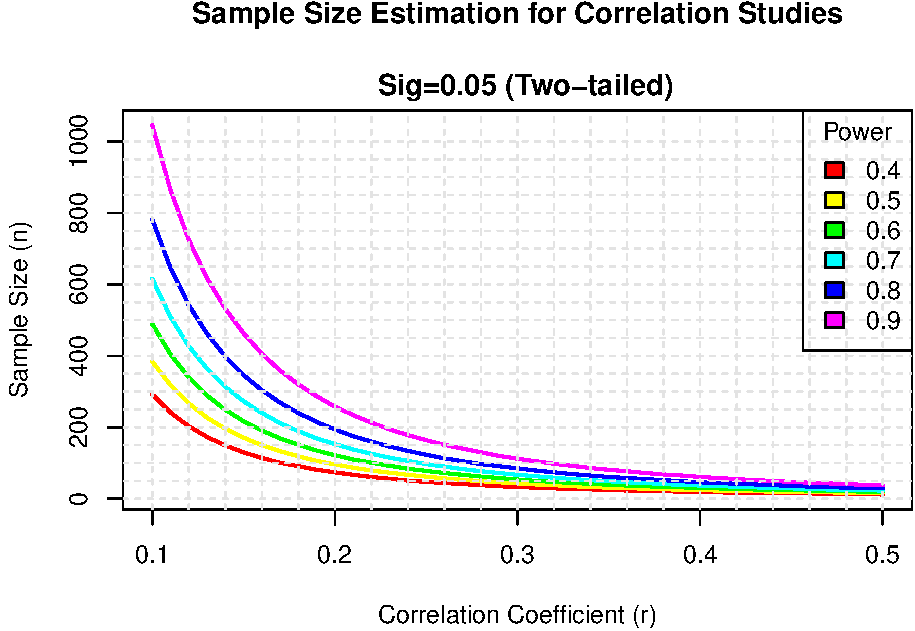
\includegraphics{index_files/figure-latex/power-1.pdf}

This a plot of power rates against these other variables. A large effect
(r \textasciitilde{} 0.5) is detectable with a sample of any size. But
only large samples have the power to detect a statistically significant
(p \textless{} .05) small correlation (r = 0.1).

\begin{center}\rule{0.5\linewidth}{0.5pt}\end{center}

\hypertarget{collecting-your-data}{%
\chapter{Collecting your Data}\label{collecting-your-data}}

\hypertarget{data-sources}{%
\section{Data Sources}\label{data-sources}}

For collecting data from Epic, it might be helpful to have a sense of
the landscape of its different databases. There are three primary
databases:

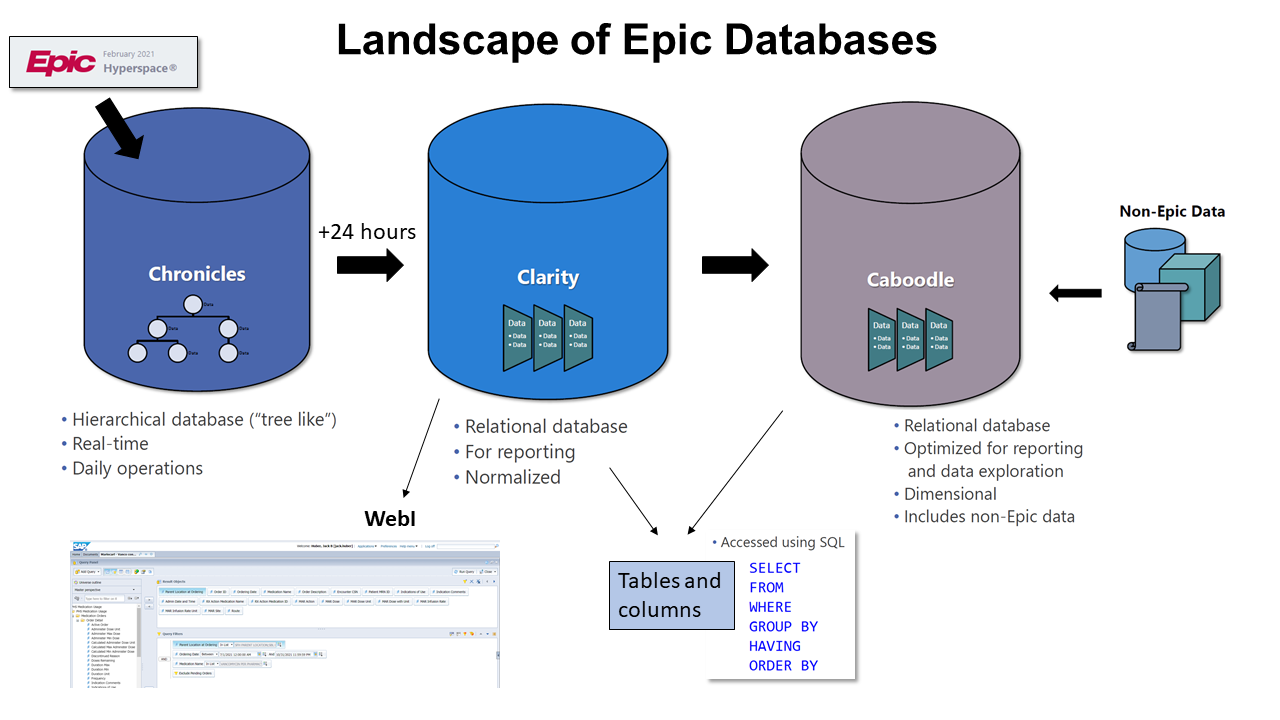
\includegraphics{EpicDataLandscape.png}

\textbf{Chronicles}. This is the database that is collecting data from
Hyperspace in real time. For reporting, Reporting Workbench pulls data
directly from Chronicles, but it is otherwise not designed very well for
historical reporting.

\textbf{Clarity}. This is the primary relational database for reporting
Epic data. Through a nightly process known as ETL
(``extract-transform-load''), Clarity extracts data from Chronicles and
stores it in a thousand bazillion tables (think ``spreadsheets''). To
pull data for a report from Clarity is to identify the correct tables
and fields and to write a SQL query to join the tables, apply the
appropriate selection criteria, and report the appropriate fields.

\textbf{Caboodle}. This a relatively new relational database that
functions essentially the same as Clarity but is designed to be much
easier to use. Caboodle uses fewer tables derived from myriad Clarity
tables which vastly simplifies the work and complexity of writing a SQL
query. The down side is not all Clarity data are in Caboodle.

\hypertarget{granularity-of-data}{%
\section{Granularity of data}\label{granularity-of-data}}

Granularity means two related things. One is the size of the data point
which is to say what context it provides for other, smaller, data
points. The other is, essentially this question: What does a row in the
spreadsheet mean? There are several different levels of granularity:

\textbf{Patient-level data}. A patient has a unique ID number: the MRN.
No two patients have the same MRN. When it comes to mining Epic data for
the research project, the patient list is perhaps the most important:
the resident needs a ``patient list''. When it comes to data mining, the
patient ``level'' is context to more granular data in the sense that a
patient can have multiple encounters - and thus multiple Encounter CSNs
``within'' the same Patient MRN.

\textbf{Encounter-level data}. The unique Epic ID number for the
encounter is the CSN. The encounter is context to more granular data
such as a treatment regimen of a particular medicine. Multiple drug
administrations can occur ``within'' an encounter CSN.

\textbf{Medication administration level data}. This is possibly the
lowest level and the most granular data. In Caboodle, each
administration of a medicine has a unique ID number and is time-stamped.
My queries to date have been for counts of medicine administrations, or
firsts, lasts, minimums and maximum doses within a hospital encounter or
ICU stay.

\textbf{Lab results level data}. Lab data is similar to medicine
administration data because, again in Caboodle, each lab result is has
its own unique ID number and is time-stamped. There can be a great many
lab results within a hospital encounter. My queries to date have been
for counts of lab results, or firsts, lasts, minimums and maximum values
within a hospital encounter or ICU stay.

The resident data collection form is designed for patient level data;
each row in the spreadsheet captures the experience of a hospital
encounter. It can also be helpful to report the medicine administration
and lab result data sorted chronologically by patient and encounter.

\hypertarget{advice-for-data-collection-and-management}{%
\section{Advice for Data Collection and
Management}\label{advice-for-data-collection-and-management}}

\textbf{Be proactive}. As you begin to decide what data to collect,
submit your project plan and requests for data in writing to me (Jack)
as soon as possible. This is so I can have a bit of time to understand
your project, do some discovery in Caboodle or Clarity, and note any
questions. Then meet with me via Teams to get on the same page.

\textbf{Devise a system for organizing your data}. By this I mean
version control. This data collection process is iterative. You will ask
for data and I'll write a SQL query that produces an Excel workbook of
data. That's one iteration. In all likelihood you'll need a revision or
two. Upon receiving your feedback I'll edit my query and produce for you
a new set of data to replace the first set. That's the second iteration.
The more iterations, the more data, the more potential for multiple
versions and data overload. And I may not be able to do more than a few
iterations. I can work on some best practices to help us through this.
Stay tuned.

\textbf{There is no substitute for chart review}. Some fraction of
resident research data can come from Epic data mining, but it still
needs to be validated with careful chart review. And some data which are
very difficult to mine or to query into the correct format may have to
come from chart review.

\begin{center}\rule{0.5\linewidth}{0.5pt}\end{center}

\hypertarget{analyzing-your-data}{%
\chapter{Analyzing your Data}\label{analyzing-your-data}}

You have data. Congratulations! Let's analyze!

\hypertarget{preparing-your-data-for-analysis}{%
\section{Preparing your data for
analysis}\label{preparing-your-data-for-analysis}}

The first step is to complete a number of tasks to prepare your data for
analysis. One data matrix. See the exemplar.

\hypertarget{choosing-appropriate-statistics}{%
\section{Choosing appropriate
statistics}\label{choosing-appropriate-statistics}}

It is important to know the measurement level of your variables. How do
you express the outcome by which to compare your pre- and post- samples?
Is it\ldots{}

\begin{itemize}
\tightlist
\item
  Mortality rate (\% surviving)? In such a case you would be comparing
  two proportions.
\item
  ``Time to\ldots{}'' a therapeutic level? In such a case you would be
  comparing two different quantities of time.
\end{itemize}

\textbf{Odds ratios / Logistic regression}. Some outcomes are binary.
Yes or no. Something happened or it didn't. Treatment worked or it did
not. For projects with binary outcomes, the researcher will want to
consider comparing odds ratios. Logistic regression would be the
appropriate technique for modeling differences between the pre- and
post-implementation groups in whether patients landed in one category or
the other.

\textbf{Chi-square test of independence}. Some outcomes are categorical.
There is no ``more'' or ``less'' but rather different categories of
outcomes. For projects with categorical outcomes, the researcher will
want to consider using chi-square tests of independence.

\textbf{Two-sample t-test}.

\textbf{Z test of the difference of proportions}.

\textbf{Cohen's \emph{d} effect size}.

\begin{center}\rule{0.5\linewidth}{0.5pt}\end{center}

\hypertarget{reporting-your-results}{%
\chapter{Reporting your Results}\label{reporting-your-results}}

\hypertarget{advice-on-graphs}{%
\section{Advice on graphs}\label{advice-on-graphs}}

\hypertarget{advice-on-tables}{%
\section{Advice on tables}\label{advice-on-tables}}

\begin{center}\rule{0.5\linewidth}{0.5pt}\end{center}

  \bibliography{bibfile.bib,packages.bib}

\end{document}
